\documentclass[12pt]{report}
\usepackage[utf8]{inputenc}
\usepackage[russian]{babel}
%\usepackage[14pt]{extsizes}
\usepackage{listings}
\usepackage{graphicx}
\usepackage{amsmath,amsfonts,amssymb,amsthm,mathtools} 
\usepackage{pgfplots}
\usepackage{filecontents}
\usepackage{float}
\usepackage{comment}
\usepackage{indentfirst}
\usepackage{caption}
\usepackage{eucal}
\usepackage{enumitem}
%s\documentclass[openany]{book}
\frenchspacing

\usepackage{indentfirst} % Красная строка

\usetikzlibrary{datavisualization}
\usetikzlibrary{datavisualization.formats.functions}

\usepackage{amsmath}


% Для листинга кода:
\lstset{ %
	language=c,                 % выбор языка для подсветки (здесь это С)
	basicstyle=\small\sffamily, % размер и начертание шрифта для подсветки кода
	numbers=left,               % где поставить нумерацию строк (слева\справа)
	numberstyle=\tiny,           % размер шрифта для номеров строк
	stepnumber=1,                   % размер шага между двумя номерами строк
	numbersep=5pt,                % как далеко отстоят номера строк от подсвечиваемого кода
	showspaces=false,            % показывать или нет пробелы специальными отступами
	showstringspaces=false,      % показывать или нет пробелы в строках
	showtabs=false,             % показывать или нет табуляцию в строках
	frame=single,              % рисовать рамку вокруг кода
	tabsize=2,                 % размер табуляции по умолчанию равен 2 пробелам
	captionpos=t,              % позиция заголовка вверху [t] или внизу [b] 
	breaklines=true,           % автоматически переносить строки (да\нет)
	breakatwhitespace=false, % переносить строки только если есть пробел
	escapeinside={\#*}{*)}   % если нужно добавить комментарии в коде
}


\usepackage[left=2cm,right=2cm, top=2cm,bottom=2cm,bindingoffset=0cm]{geometry}
% Для измененных титулов глав:
\usepackage{titlesec, blindtext, color} % подключаем нужные пакеты
\definecolor{gray75}{gray}{0.75} % определяем цвет
\newcommand{\hsp}{\hspace{20pt}} % длина линии в 20pt
% titleformat определяет стиль
\titleformat{\chapter}[hang]{\Huge\bfseries}{\thechapter\hsp\textcolor{gray75}{|}\hsp}{0pt}{\Huge\bfseries}


% plot
\usepackage{pgfplots}
\usepackage{filecontents}
\usetikzlibrary{datavisualization}
\usetikzlibrary{datavisualization.formats.functions}

\newcommand{\imgw}[3] {
	\begin{figure}[h]
		\centering
		\includegraphics[width=#1]{#2}
		\caption{#3}
		\label{img:#2}
	\end{figure}
}

\begin{document}
	%\def\chaptername{} % убирает "Глава"
	\thispagestyle{empty}
	\begin{titlepage}
		\noindent \begin{minipage}{0.15\textwidth}
			
\includegraphics[width=\linewidth]{img/b_logo}
		\end{minipage}
		\noindent\begin{minipage}{0.9\textwidth}\centering
			\textbf{Министерство науки и высшего образования Российской Федерации}\\
			\textbf{Федеральное государственное бюджетное образовательное учреждение высшего образования}\\
			\textbf{~~~«Московский государственный технический университет имени Н.Э.~Баумана}\\
			\textbf{(национальный исследовательский университет)»}\\
			\textbf{(МГТУ им. Н.Э.~Баумана)}
		\end{minipage}
		
		\noindent\rule{18cm}{3pt}
		\newline\newline
		\noindent ФАКУЛЬТЕТ $\underline{\text{«Информатика и системы управления»}}$ \newline\newline
		\noindent КАФЕДРА $\underline{\text{«Программное обеспечение ЭВМ и информационные технологии»}}$\newline\newline\newline\newline\newline
		
		\begin{center}
			\noindent\begin{minipage}{1.1\textwidth}\centering
				\Large\textbf{Отчет по лабораторной работе №1}\newline
				\textbf{по дисциплине <<Математическая статистика>>}\newline
			\end{minipage}
		\end{center}
		
		\noindent\textbf{Тема} $\underline{\text{Гистограмма и эмпирическая функция распределения}}$\newline\newline
		\noindent\textbf{Студент} $\underline{\text{Леонов В.В.}}$\newline\newline
		\noindent\textbf{Группа} $\underline{\text{ИУ7-66Б}}$\newline\newline
		\noindent\textbf{Оценка (баллы)} $\underline{\text{~~~~~~~~~~~~~~~~~}}$\newline\newline
		\noindent\textbf{Преподаватель} $\underline{\text{Власов П.А., Андреева Т.В.}}$\newline\newline\newline
		
		\begin{center}
			\vfill
			Москва~---~\the\year
			~г.
		\end{center}
	\end{titlepage}
	
\chapter*{Постановка задачи}

\textbf{Цель работы:} построение гистограммы и эмпирической функции распределения.

\begin{enumerate}
	\item Для выборки объёма $n$ из генеральной совокупности $X$ реализовать в виде программы на ЭВМ
	\begin{enumerate}
		\item вычисление максимального значения $M_{\max}$ и минимального значения $M_{\min}$;
		\item размаха $R$ выборки;
		\item вычисление оценок $\hat\mu$ и $S^2$ математического ожидания $MX$ и дисперсии $DX$;
		\item группировку значений выборки в $m = [\log_2 n] + 2$ интервала;
		\item построение на одной координатной плоскости гистограммы и графика функции плотности распределения вероятностей нормальной случайной величины с математическим ожиданием $\hat{\mu}$ и дисперсией $S^2$;
		\item построение на другой координатной плоскости графика эмпирической функции распределения и функции распределения нормальной случайной величины с математическим ожиданием $\hat{\mu}$ и дисперсией $S^2$.
	\end{enumerate}
	\item Провести вычисления и построить графики для выборки из индивидуального варианта.
\end{enumerate}

\textbf{Вариант 9:}

X = (-8.47, -7.45, -7.12, -8.30, -8.15, -6.01, -5.20, -7.38, -6.76, -9.18, -6.00, -8.08, -7.96, -8.34, -6.82, -8.46, -8.07, -7.04, -7.24, -8.16, -8.20, -8.27, -7.79, -7.37, -7.02, -7.13, -6.99, -7.65, -8.18, -6.71, -8.41, -6.71, -7.04, -9.15, -7.74, -10.11, -8.20, -7.07, -7.63, -8.99, -6.62, -6.23, -7.13, -6.41, -7.06, -7.72, -8.44, -8.85, -8.02, -6.98, -6.08, -7.20, -7.48, -7.82, -9.19, -8.31, -7.95, -7.97, -6.66, -6.59, -9.10, -7.87, -9.02, -8.77, -7.62, -9.44, -8.05, -7.60, -7.33, -6.94, -8.51, -7.39, -6.44, -8.88, -8.21, -7.66, -6.91, -8.39, -7.37, -7.26, -6.04, -7.58, -7.28, -7.02, -7.10, -7.33, -8.63, -8.21, -7.12, -8.11, -9.03, -8.11, -8.79, -9.22, -7.32, -5.97, -7.26, -6.39, -7.64, -8.38, -7.67, -7.70, -7.70, -8.95, -6.25, -8.09, -7.85, -8.10, -7.73, -6.78, -7.78, -8.20, -8.88, -8.51, -7.45, -7.14, -6.63, -7.38, -7.72, -6.25)

\clearpage

\chapter*{Общие теоретические сведения}

\section*{Формулы для вычисления величин}

Пусть $\vec x$ -- выборка из генеральной совокупности $X$. 

\subsection*{Минимальное и максимальное значения выборки}
\begin{equation}
	\begin{aligned}
		M_{\max} = x_{(n)}\\
		M_{\min} = x_{(1)},
	\end{aligned}
\end{equation}

где $x_{(i)}$ -- элемент вариационного ряда.

\subsection*{Размах выборки}
\begin{equation}
	R = M_{\max} - M_{\min}.
\end{equation}


\subsection*{Оценки математического ожидания и дисперсии}
\begin{equation}
	\begin{aligned}
		\hat\mu(\vec x_n) &= \frac 1n \sum_{i=1}^n x_i\\
		S^2(\vec x_n) &= \frac 1{n-1} \sum_{i=1}^n (x_i-\overline x_n)^2,
	\end{aligned}
\end{equation}

где $\overline x_n = \hat\mu(\vec x_n)$.

\newpage

\section*{Определение эмпирической плотности и гистограммы}

Пусть $\vec x = (x_1, ..., x_n)$ -- выборка из генеральной совокупности $X$. Если объем $n$ этой выборки велик, то значения $x_i$ группируют в интервальный статистический ряд. Для этого отрезок $J = [x_{(1)}, x_{(n)}]$ делят на $m$ равновеликих частей:

\begin{equation*}
	J_i = [x_{(1)} + (i - 1) \cdot \Delta, x_{(1)} + i \cdot \Delta), i = \overline{1; m - 1}
\end{equation*}

\begin{equation*}
	J_{m} = [x_{(1)} + (m - 1) \cdot \Delta, x_{(n)}]
\end{equation*}

\begin{equation*}
	\Delta = \frac{|J|}{m} = \frac{x_{(n)} - x_{(1)}}{m}
\end{equation*}

Интервальным статистическим рядом называют таблицу:

\begin{table}[htb]
	\centering
	\begin{tabular}{|c|c|c|c|c|}
		\hline
		$J_1$ & ... & $J_i$ & ... & $J_m$ \\
		\hline
		$n_1$ & ... & $n_i$ & ... & $n_m$ \\
		\hline
	\end{tabular}
\end{table}

где $n_i$ -- количество элементов выборки $\vec x$, которые $\in J_i$.

Обычно выборку разбивают на $m=[\log_2n]+2$ интервалов, где $n$ -- размер выборки.

Гистограмма -- это график эмпирической плотности. 

\textit{Эмпирической плотностью}, отвечающей выборке $\vec x$, называют функцию:
\begin{equation}
	\hat f(x) =
	\begin{cases}
		\frac{n_i}{n \Delta}, x \in J_i, i = \overline{1; m} \\
		0, \text{иначе} \\
	\end{cases}
\end{equation}

где $J_i$ -- полуинтервал статистического ряда, $n_i$ -- количество элементов выборки, входящих в полуинтервал, $n$ -- количество элементов выборки.


\section*{Определение эмпирической функции распределения}

Пусть $\vec x = (x_1, ..., x_n)$ -- выборка из генеральной совокупности $X$. Обозначим $n(x, \vec x)$ -- число элементов вектора $\vec x$, которые имеют значения меньше $x$.

\textit{Эмпирической функцией распределения} называют функцию $F_n: \mathbb{R} \to \mathbb{R}$, определенную как: 

\begin{equation}
	F_n(x) = \frac{n(x, \vec x)}{n}
\end{equation}

\chapter*{Ход работы}
Для решения поставленной задачи была использованна программа \textit{MATLAB 2022a}.

\subsection*{Листинг программы}
\begin{lstlisting}
function main()
	function myhist(X, bins, counts, R, m)
		n = length(X);
		delta = R / m;
		middles = zeros(1, m);
		xx = zeros(1, m);
		
		for i = 1:m
			xx(i) = counts(i) / (n * delta);
		end
		
		for i = 1:m
			middles(i) = bins(i) + (delta/2);
		end
		
		fprintf("    delta: %f\n", delta);
		fprintf("    hist coords:\n");
		
		for i = 1:m
			fprintf("    [%d] : %f %f\n", i,middles(i), xx(i));
		end
		
		fprintf("    hist_s = %f\n", sum(xx) * delta);
		set(gca, "xlim", [min(bins) - 1, max(bins) + 1]);
		bar(middles, xx,1, "facecolor", "b", "edgecolor", "w");
		
		X_range = m_min:(sigma / 100):m_max;
		X_pdf = normpdf(X_range, mx, sigma);
		plot(X_range, X_pdf, "r");
		end

	function mycdf(X, bins, counts)
		n = length(X);
		xx = zeros(1, m + 3);
		
		bins = [(min(bins) - 0.5) bins (max(bins) + 1)];
		counts = [0 counts 0];
		
		m = m + 2;
		acc = 0;
		
		for i = 2:m
			acc = acc + counts(i);
			xx(i) = acc / n;
		end
		
		xx(m + 1) = 1;
		
		X_n = (min(X) - 0.5):(sigma / 100):(max(X) + 1.5);
		X_cdf = normcdf(X_n, mx, sigma);
		plot(X_n, X_cdf, "r");
		
		for i = 2:m
			fprintf("x = %f : F(x) = %f\n", bins(i), xx(i));
		end
		
		set(gca, "ylim", [0, 1.1]);
		stairs(gca, bins, xx, "b");
	end

	X = [-8.47, -7.45, -7.12, -8.30, -8.15, -6.01, -5.20, -7.38, -6.76, -9.18, -6.00, -8.08, -7.96, -8.34, -6.82, -8.46, -8.07, -7.04, -7.24, -8.16, -8.20, -8.27, -7.79, -7.37, -7.02, -7.13, -6.99, -7.65, -8.18, -6.71, -8.41, -6.71, -7.04, -9.15, -7.74, -10.11, -8.20, -7.07, -7.63, -8.99, -6.62, -6.23, -7.13, -6.41, -7.06, -7.72, -8.44, -8.85, -8.02, -6.98, -6.08, -7.20, -7.48, -7.82, -9.19, -8.31, -7.95, -7.97, -6.66, -6.59, -9.10, -7.87, -9.02, -8.77, -7.62, -9.44, -8.05, -7.60, -7.33, -6.94, -8.51, -7.39, -6.44, -8.88, -8.21, -7.66, -6.91, -8.39, -7.37, -7.26, -6.04, -7.58, -7.28, -7.02, -7.10, -7.33, -8.63, -8.21, -7.12, -8.11, -9.03, -8.11, -8.79, -9.22, -7.32, -5.97, -7.26, -6.39, -7.64, -8.38, -7.67, -7.70, -7.70, -8.95, -6.25, -8.09, -7.85, -8.10, -7.73, -6.78, -7.78, -8.20, -8.88, -8.51, -7.45, -7.14, -6.63, -7.38, -7.72, -6.25];
	m_max = max(X);
	m_min = min(X);
	fprintf("(a) \n");
	fprintf("    max_value = %f\n", m_max);
	fprintf("    min_value = %f\n", m_min);
	fprintf("----------------------------------------\n");
	
	r = m_max - m_min;
	fprintf("(b) \n");
	fprintf("    r = %f\n", r);
	fprintf("----------------------------------------\n");
	
	n = length(X);
	mx = sum(X) / n;
	dx = sum((X - mx).^2) / (n - 1);
	sigma = sqrt(dx);
	
	fprintf("(c) \n");
	fprintf("    mx = %f\n", mx);
	fprintf("    dx = %f\n", dx);
	fprintf("----------------------------------------\n");
	
	m = floor(log2(n)) + 2;
	bins = [];
	cur = m_min;
	
	for i = 1:(m + 1)
		bins(i) = cur;
		cur = cur + r / m;
	end
	
	eps = 1e-6;
	counts = [];
	j = 1;
	
	for i = 1:(m - 1)
		cur_count = 0;
		for j = 1:n
			if (bins(i) < X(j) || abs(bins(i) - X(j)) < eps) && X(j) < bins(i + 1)
				cur_count = cur_count + 1;
			end
		end
		counts(i) = cur_count;
	end
	
	cur_count = 0;
	
	for j = 1:n
		if (bins(m) < X(j) || abs(bins(m) - X(j)) < eps) && (X(j) < bins(m + 1) || abs(bins(m + 1) - X(j)) < eps)
			cur_count = cur_count + 1;
		end
	end
	
	counts(m) = cur_count;
	
	fprintf("(d)\n");
	
	for i = 1:(m)
		fprintf("    [%f : %f) - %d values.\n", bins(i), bins(i + 1), counts(i));
	end
	
	fprintf("----------------------------------------\n");
	
	fprintf("(e) \n");
	
	figure;
	hold on;
	grid on;
	myhist(X, bins, counts, r, m);
	xlabel('X')
	ylabel('P')
	hold off;
	
	fprintf("----------------------------------------\n");
	
	fprintf("(f) \n");
	
	figure;
	hold on;
	grid on;
	mycdf(X, bins, counts);
	xlabel('X')
	ylabel('F')
	hold off;
end
\end{lstlisting}

\subsection*{Результат работы программы}
\begin{equation*}
	M_{\min} = -10.110000 \\
\end{equation*}
\begin{equation*}
	M_{\max} = -5.200000 \\
\end{equation*}
\begin{equation*}
	R = 4.910000 \\
\end{equation*}
\begin{equation*}
	\hat\mu(\vec x_n) = -7.660917 \\
\end{equation*}
\begin{equation*}
	S^2(\vec x_n) = 0.777892 \\
\end{equation*}
\begin{equation*}
	m = 8
\end{equation*}

\newpage

\captionsetup{justification=centering}

\begin{figure}[h!]
	\centering
	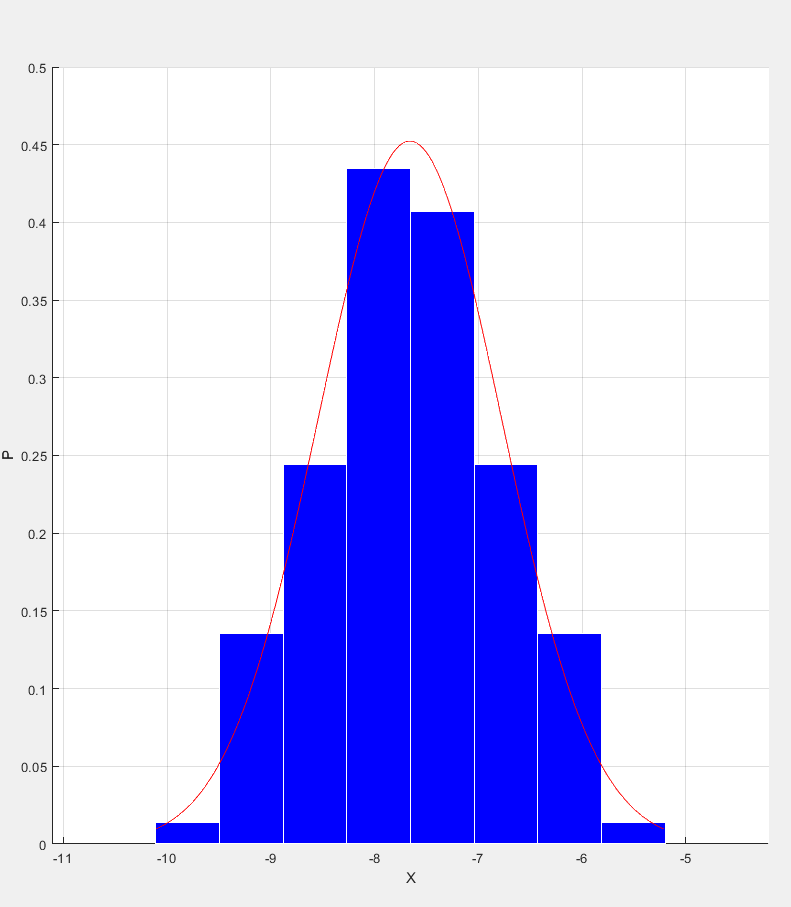
\includegraphics[width=\textwidth]{img/hist}
	\caption{Гистограмма и график функции плотности распределения вероятностей нормальной случайной величины с выборочными мат. ожиданием и дисперсией}
\end{figure}

\newpage

\begin{figure}[h!]
	\centering
	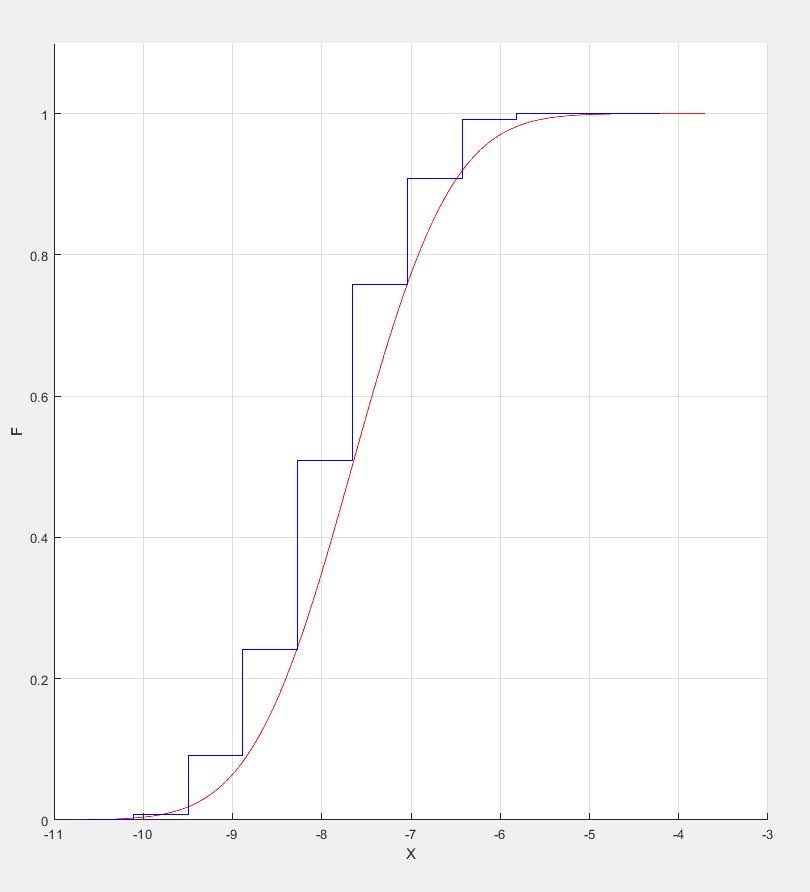
\includegraphics[width=\textwidth]{img/cdf}
	\caption{График эмперической функции распределения и функции распределения нормальной случайной величины с выборочными мат. ожиданием и дисперсией}
\end{figure}



\bibliographystyle{utf8gost705u}  % стилевой файл для оформления по ГОСТу
\bibliography{51-biblio}          % имя библиографической базы (bib-файла)
	
\end{document}
